\section{Risultati degli algoritmi}
Questa sezione risponderà alla Domanda 1: verranno riportati sotto forma di tabella i risultati dei costi per il problema TSP dei grafi richiesti, il tempo di esecuzione di ogni algoritmo e l'errore relativo rispetto alla soluzione esatta. I risultati ottenuti,poi, verranno opportunamente discussi.

\subsection{Domanda 1}
Eseguite i tre algoritmi che avete implementato (Held-Karp, euristica costruttiva e 2-approssimato) sui 13 grafi del dataset. Mostrate i risultati che avete ottenuto in una tabella come quella sottostante. Le righe della corrispondono alle istanze del problema. Le colonne mostrano, per ogni algoritmo, il peso della soluzione trovata, il tempo di esecuzione e l'errore relativo calcolato come $(SoluzioneTrovata - SoluzioneOttima)/SoluzioneOttima$. Potete aggiungere altre informazioni alla tabella che ritenete interessanti. 
\image{1}{estab}{Esempio di tabella riportante i risultati ottenuti}
\subsubsection{Svolgimento}
\label{tab}
\begin{center}
	\scriptsize
	\begin{longtable}{|c|c|c|c|c|c|c|c|c|c|}	
	\hline
		\multirow{2}{*}{\textbf{Istanza}} & \multicolumn{3}{c|}{\textbf{Held-Karp}} & \multicolumn{3}{c|}{\textbf{Cheapest Insertion}} & \multicolumn{3}{c|}{\textbf{TriangleTSP}} \\ \cline{2-10}
		 &\textbf{Soluzione}& \textbf{Tempo (s)} & \textbf{Errore (\%)} & \textbf{Soluzione}& \textbf{Tempo (s)} & \textbf{Errore (\%)} & \textbf{Soluzione}& \textbf{Tempo (s)} & \textbf{Errore (\%)} \\ \hline
		\endfirsthead
		\multicolumn{10}{|c|}%
		{\tablename\ \thetable\ \ --\  \textit{continuazione della pagina precedente}} \\
		\hline
		\multirow{2}{*}{\textbf{Istanza}} & \multicolumn{3}{c|}{\textbf{Held-Karp}} & \multicolumn{3}{c|}{\textbf{Held-Karp}} & \multicolumn{3}{c|}{\textbf{Held-Karp}} \\ \cline{2-10}
		 &\textbf{Soluzione}& \textbf{Tempo (s)} & \textbf{Errore (\%)} & \textbf{Soluzione}& \textbf{Tempo (s)} & \textbf{Errore (\%)} & \textbf{Soluzione}& \textbf{Tempo (s)} & \textbf{Errore (\%)} \\ \hline
		\endhead
		\hline \multicolumn{10}{|r|}{\textit{Continua nella pagina seguente}} \\
		\endfoot
		\endlastfoot
		berlin52.tsp & 17441 & 120,0174 & 131,25 & 9004 & 0,0096 & 19,38& 10402 &0,0074 &37.92 \\ \hline
		burma14.tsp & 3323 & 0,2029 & 0,0 & 3588 & 0,0003 & 7,97 &4003 & 0,0002&20.46\\ \hline
		ch150.tsp & 47935 & 120,95 & 634,30 & 7998 & 0,0678 & 22,52 &9126 &0,02343 &39.80  \\ \hline
		d493.tsp & 111947 & 120,4769&219,83 & 39969 & 0,4976 & 14,19 &45300 &0,1063 &29.42 \\ \hline
		dsj1000.tsp & \scriptsize 551274242 &120,0012 &2854,36 & 22291165 & 7,5382 & 19,46 &25526005 &0,5358 &36.80 \\ \hline
		eil51.tsp&986 &120,0005 &131,46 & 494 &0,0006 & 15,96 &614 & 0,0009 &44.13 \\ \hline
		gr202.tsp&55127 &119,9998 &37,26 & 46480 & 0,0406 & 15,74 &52615 & 0,0189& 31.01\\ \hline
		gr229.tsp&176212 & 120,0008&30,91 & 153896 & 0,0493 & 14,33 &179335 &0,0249 &33.23 \\ \hline
		kroA100.tsp& 164223 & 120,0003 & 671,65 & 24942 & 0,0038 & 17,20&30536 &0,0014 &43.48 \\ \hline
		kroD100.tsp& 144125 &120,0012 &576,83 &25204 & 0,0036 & 18,36 &28599 &0,0017 &34.31 \\ \hline
		pcb442.tsp& 202233&120,4061 &298,27 & 60834 & 0,3954 & 19,80 &68841 &0,0901 & 35.57\\ \hline
		ulysses16.tsp&6859 &0,5584 & 0,0 & 7368 & 0,0001 & 7,42&7788 & 0,0001 & 13.54\\ \hline
		ulysses22.tsp&7013 &59,4115 &0,0 &  7709 & 0,0001 & 9,92 &8308 &0,0001 &18.47 \\ \hline		 
     \caption{Risultati dei tre algoritmi implementati rispetto alla domanda 1}
     \label{results}
	\end{longtable}
\end{center}\vspace{-40pt}

\subsection{Domanda 2}
Commentate i risultati che avete ottenuto: come si comportano gli algoritmi rispetto alle varie istanze? C'è un algoritmo che riesce sempre a fare meglio degli altri rispetto all'errore di approssimazione? Quale dei tre algoritmi che avete implementato è più efficiente? 

\subsubsection{Svolgimento}
\begin{itemize}
	\item \textbf{Come si comportano gli algoritmi rispetto alle varie istanze?}
	\begin{itemize}
		\item \texttt{HeldKarp}: nelle istanze fino di 14 e 16 nodi l'algoritmo termina quasi immediatamente, restituendo la soluzione ottima. Nell'istanza con 22 nodi impiega poco meno di un minuto per trovarla. Per tutte le altre istanze, occorre dare un tempo limite a disposizione dell'algoritmo in quanto impiegherebbe decisamente troppo tempo per calcolare la soluzione ottima. Pur interrompendo la computazione, non è possibile fare alcuna previsione sulla qualità della soluzione ritornata calcolata fino a quel punto, che arriva anche ad essere del 2854,36\% nel caso di \texttt{disj1000.tsp}.
		\item \texttt{CheapestInsertion}: l'algoritmo ritorna una soluzione 2-approssimata\footnote{grazie al vincolo rispettato di disuguaglianza triangolare} quasi immediatamente, fatta eccezione per \texttt{disj1000.tsp} che impiega circa 7,5 secondi. Ogni soluzione ritornata ha un errore che appartiene all'intervallo $[7.97 - 22.52]$\%: in media ogni soluzione ha un errore relativo del 15,56\% rispetto alla sua soluzione ottima. Un notevole risultato, tenendo conto che potrebbe teoricamente ritornare una soluzione con errore relativo al più del 200\%.
		\item \texttt{TriangleTSP}: l'algoritmo ritorna una soluzione 2-approssimata quasi immediatamente per tutte le istanze del dataset. Ogni soluzione ritornata possiede un errore relativo che appartiene all'intervallo $[13.54 - 44.13]$\%: in media ogni soluzione ha un errore relativo del 30.74\%. Un risultato quasi doppio rispetto all'euristica \texttt{CheapestInsertion}: ulteriori chiarimenti saranno forniti nella sezione \S\ref{ci-ttsp}
	\end{itemize}
	\item \textbf{C'è un algoritmo che riesce sempre a fare meglio degli altri rispetto all'errore di approssimazione?}
	\begin{itemize}
		\item \texttt{HeldKarp} riesce sempre a fare meglio di \texttt{CheapestInsertion} e \texttt{TriangleTSP} nelle istanze con meno di 23 nodi, vale a dire \texttt{burma14.tsp, ulysses16.tsp} e \texttt{ulysses22.tsp} perché riesce a trovare la soluzione ottima. Per tutte le altre istanze del dataset, \texttt{CheapestInsertion} riesce sempre a trovare una soluzione più vicina alla soluzione ottima rispetto agli altri due algoritmi implementati: il perché di questo dato di fatto non è ci è perfettamente chiaro. Abbiamo pensato che potrebbe essere perché... %TODO
	\end{itemize}
	\item \textbf{Quale dei tre algoritmi che avete implementato è più efficiente?}
	\begin{itemize}
		\item Considerando il termine \quotes{efficienza} ed il suo significato in campo informatico, inteso come la capacità di utilizzare meno risorse\footnote{tempo di utilizzo della CPU e memoria} possibile durante la sua esecuzione, l'algoritmo più efficiente si rivela essere \texttt{TriangleTSP} perché è corretto rispetto al vincolo di 2-approssimazione ed impiega meno risorse di \texttt{CheapestInsertion}. Quest'ultimo, tuttavia, riesce a trovare una soluzione quasi il doppio più accurata del primo, a fronte di utilizzi di risorse più che accettabili per le istanze di TSP fornite. \`{E} per questo che ci sentiamo di dire che l'algoritmo che, mediamente, riesce a combinare \textbf{efficienza} ed \textbf{efficacia} meglio di tutti sia proprio \texttt{CheapestInsertion}.
	\end{itemize}
\end{itemize}


\paragraph{Discussione su \texttt{CheapestInsertion} e \texttt{TriangleTSP}} \label{ci-ttsp}
Entrambi gli algoritmi sono una 2-approssimazione per TSP, ma riportano risultati differenti: \texttt{CheapestInsertion} richiede più tempo per essere eseguito rispetto a \texttt{TriangleTSP}, ma ottiene un errore relativo minore.\eqcapo 
Per capire dunque quale dei due algoritmi sia più efficiente ed efficace, è possibile osservare gli istogrammi in Figura~\ref{confronto} che mostrano prima la differenza del tempo di esecuzione dei due algoritmi su scala logaritmica per i vari grafi, poi il tempo di esecuzione su una scala normale ed infine il rispettivo errore relativo. Confrontando il primo e terzo istogramma è possibile vedere come per un aggiunta di tempo di computazione relativamente basso si ottiene un notevole miglioramento per l'errore relativo, infatti \texttt{TriangleTSP} raggiunge in media un errore relativo più alto ($\sim$32\%) rispetto a \texttt{CheapestInsertion} ($\sim$16\%). Se si osserva il secondo istogramma si può vedere come con grafi di taglia maggiore il tempo di esecuzione per \texttt{CheapestInsertion} aumenti esponenzialmente rispetto a \texttt{TriangleTSP}, basti osservare il tempo di esecuzione per i grafi \texttt{d449.tsp} e \texttt{dsj1000.tsp}: dunque per grafi di grande taglia è consigliabile utilizzare \texttt{TriangleTSP}, altrimenti \texttt{CheapestInsertion}.

\begin{figure}[H]
	\centering
	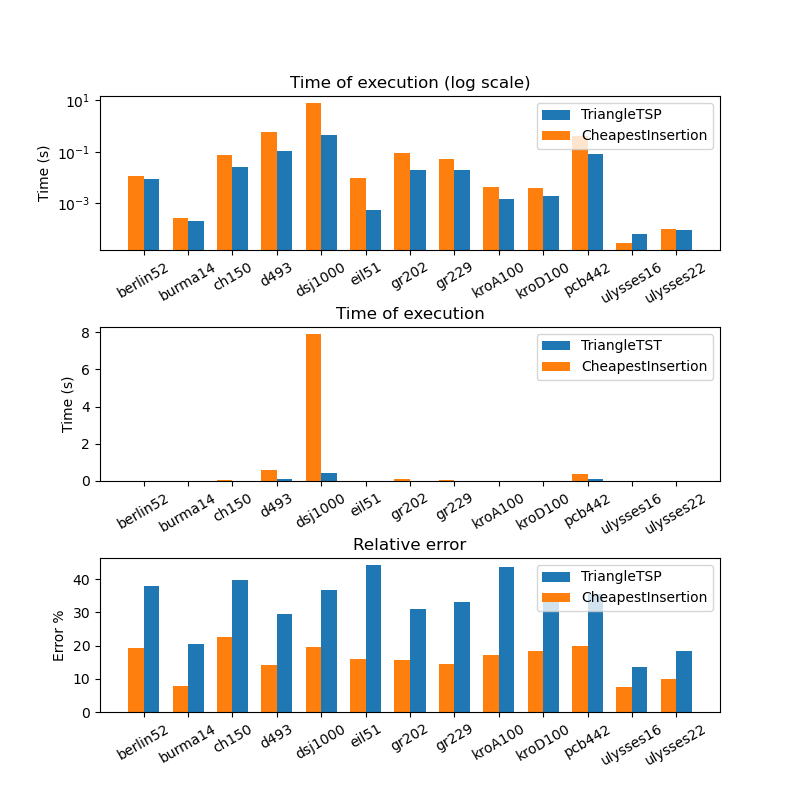
\includegraphics[width=\textwidth]{confronto}
	\caption{Confronto tra \texttt{CheapestInsertion} e \texttt{TriangularTSP}}
	\label{confronto}
\end{figure}

\newpage
\section{Descrizione degli algoritmi}
\subsection{CheapestInsertion}

L'algoritmo opera con l'assunzione che il grafo dato rispetti la disuguaglianza triangolare, inserendo iterativamente un nodo $k$ all'interno del circuito parziale per la soluzione a TSP per $n-2, n=|V|$ volte con $V$ l'insieme dei nodi del grafo. In particolare, dato $k \notin C \subseteq V$, con $C$ l'insieme dei nodi nel circuito parziale, e i nodi $u,v \in C$ \mbox{t.c.} $(u,v)\in P$, con $P$ l'insieme dei lati nel circuito parziale, $k$ viene scelto ed inserito nel circuito parziale tra i nodi $u$ e $v$ minimizzando: $w(u,k)+w(k,v)-w(u,v)$.

La complessità dell'algoritmo si può calcolare analizzando i tre cicli \texttt{for} nell'algoritmo. Il ciclo più esterno viene eseguito $n-2$ volte. I due cicli più interni scorrono tutti i nodi $k \notin C$ e i lati $(u,v)\in P$. \'E possibile vedere come, ad ogni iterazione del ciclo \texttt{for} più esterno il numero di iterazioni dei due cicli più in interni, rispettivamente diminuiscano ed aumentino; in particolare il numero totale di iterazioni compiute dai tre cicli \texttt{for} è: $\sum_{i=2}^{n-1} (n-i)i=\frac{1}{6}(n^3-7n+6)$. Dunque l'algoritmo \texttt{CheapestInsertion} possiede una complessità di \comp{n^3}.
Questo risultato risulta evidente analizzando i tempi di risoluzione dei vari grafi in Tabella~\ref{results}, il quale aumenta esponenzialmente all'aumentare della taglia del grafo, passando dai $\sim$0.004 s per un grafo da 100 nodi, a $\sim$7.5 s per un grafo da 1000 nodi.

L'algoritmo è 2-approssimato per TSP, anche se nei grafi forniti l'errore relativo massimo è del 22\%, dimostrando dunque di essere molto efficace.

\image{1}{cheapest}{Snippet del codice per \texttt{CheapestInsertion}}

\subsection{TriangleTSP}

L'algoritmo crea il circuito per TSP attraverso la lista preordinata dei nodi del MST ottenuto dall'algoritmo \texttt{Kruskal}. Tale algoritmo costruisce un albero la cui radice è un'istanza della classe \texttt{Node}, che non ha niente a che fare con la classe \texttt{Graph} ed è utilizzata esclusivamente dall'algoritmo \texttt{Kruskal}. Un discorso analogo vale per la classe \texttt{Edge} usata solamente dall'algoritmo \texttt{Kruskal} per ottenere una lista ordinata per peso dei lati del grafo.\acapo

Dato $n=|V|$ e $m=|E|$, l'algoritmo \texttt{TriangleTSP}, dato utilizza \texttt{Kruskal}, ha una complessità \comp{m\log n}.\acapo

L'algoritmo è 2-approssimazione per TSP, e per i grafi forniti ottiene risultati con un errore relativo al massimo del 45\%, impiegando un tempo di esecuzione di $\sim$0.5 secondi. Dunque un algoritmo molto efficiente.

\image{1}{triangular}{Snipped del codice per \texttt{TriangleTSP}}
